%	!Mode::"UTF-8"
%	本模板设置改自北京大学交叉学院 王宇哲学长和北京大学化学与分子工程学院 王应泽同学的分享,特此感谢!
%	模板制作:北京大学化学与分子工程学院 王梓涵
%	Email:2100011837@stu.pku.edu.cn
%	本模板仅适用于北京大学物理化学实验报告,其他学校请自行修改
%	吐槽:Latex用于写物化实验报告还是过于繁琐了,不过还是比Word好用多了(๑•̀ㅂ•́)و✧ (此吐槽由copilot自动生成,模板作者认为word更好用)
%	本模板仅供交流学习使用,不可用作商业用途。

\documentclass[12pt]{article}

%	页面设置
\usepackage{geometry}
\geometry{left=2.5cm, right=2.5cm, top=2.5cm, bottom=2.5cm}
\usepackage{graphicx}
\usepackage{ctex}
\usepackage{fontspec}
\usepackage{setspace}
\usepackage[usenames,dvipsnames]{xcolor}
\usepackage{titlesec}

%	字体设置
\setmainfont{Times New Roman}
\setCJKmainfont{SimSun}
\setCJKsansfont{SimHei}
\setCJKmainfont[AutoFakeBold=true]{SimSun}

%	表格设置\
\usepackage{array,colortbl}
\usepackage{makecell}
\newcommand{\addcell}[2][4]{\makecell{\zihao{#1}\textsf{#2}}}
\usepackage{titlesec}
\usepackage{booktabs}
\usepackage{ragged2e} 
\usepackage{multirow}
\usepackage{tabularx}

%	设置图注、表注
\usepackage{caption}
\usepackage{bicaption}
\captionsetup{labelsep=quad, font={small, bf}, skip=2pt}
\DeclareCaptionOption{english}[]{
    \renewcommand\figurename{Fig.}
    \renewcommand\tablename{Table}
}
\captionsetup[bi-second]{english}

%	设置页眉
\usepackage{fancyhdr}
\usepackage{xpatch}
\pagestyle{fancy}
\fancypagestyle{preContent}{
    	\fancyhead[L]{\zihao{-5} 物理化学实验}
    	\fancyhead[C]{\zihao{-5} 实验三\ \ 液体饱和蒸气压的测定}
    	\fancyhead[R]{\zihao{-5} 2100011837\ 王梓涵}
		\renewcommand{\headrulewidth}{2pt}
		\renewcommand{\footrulewidth}{1pt}
		\xpretocmd\headrule{\color{BrickRed}}{}{\PatchFailed} % 设置页眉分割线颜色
		\xpretocmd\footrule{\color{BrickRed}}{}{\PatchFailed} % 设置页脚分割线颜色
}
\pagestyle{preContent}



%	设置首页页眉及取消首页页脚 若不需要首页页眉 请注释掉下列内容
\fancypagestyle{plain}{
	\fancyhead[L]{\zihao{-5} 物理化学实验}
    \fancyhead[C]{\zihao{-5} 实验三\ \ 液体饱和蒸气压的测定}
	\fancyhead[R]{\zihao{-5} 2100011837\ 王梓涵}
	\cfoot{}
}

%	设置标题格式
\titleformat*{\section}{\color{Mahogany}\zihao{4}\sffamily}
\titleformat*{\subsection}{\zihao{-4}\sffamily}
\titleformat*{\subsubsection}{\zihao{-4}\sffamily}
\titlespacing*{\section}{0pt}{10pt}{10pt}
\titlespacing*{\subsection}{0pt}{10pt}{5pt}
\titlespacing*{\subsubsection}{0pt}{10pt}{5pt}


%	设置引用格式(ACS格式规范)
%	注意:请安装JabRef
%	JabRef使用参考:https://blog.csdn.net/weixin_44191286/article/details/85698921
\usepackage[super,round,comma,compress]{natbib}

%	数学公式增强
\usepackage{amsmath}
\usepackage{amssymb}

%	单位与数学式
\usepackage{siunitx}

%	设置封面
\begin{document}
    % 标题页
    \begin{titlepage}
    	% 页眉
    	\thispagestyle{plain}
        % 校徽图片
        \begin{figure}[h]
            \centering
            \includegraphics{pku.png}
        \end{figure}
        \vspace{24pt}
        % 标题
        \centerline{\zihao{-0} \textsf{\textcolor{Mahogany}{物理化学实验报告}}}
        \vspace{40pt} % 空行
        \begin{center}
            \begin{tabular}{cp{14.1cm}}
                % 题目
                \addcell[2]{题目:} & \addcell[2]{液体饱和蒸气压的测定} \\
                \cline{2-2}
            \end{tabular}
        \end{center}
        \vspace{20pt} % 空行
        \begin{center}
            \doublespacing
            \begin{tabular}{cp{5cm}}
                % 姓名
                \addcell{姓\phantom{空格}名:\ } & \addcell{王梓涵} \\
                \cline{2-2}
                % 学号
                \addcell{学\phantom{空格}号:\ } & \addcell{2100011837}\\
                \cline{2-2}
                % 组别
                \addcell{组\phantom{空格}别:\ } & \addcell{22组 2号} \\
                \cline{2-2}
                % 实验日期
                \addcell{实验日期:\ } & \addcell{2023.11.30}\\
                \cline{2-2}
                % 室温
                \addcell{室\phantom{空格}温:\ } & \addcell{291.85\ K}\\
                \cline{2-2}
                % 大气压强
                \addcell{大气压强:\ } & \addcell{102.76\ kPa}\\
                \cline{2-2}
            \end{tabular}
            \begin{tabular*}{\textwidth}{c}
                \\ % 这是空行
                \\ % 这是空行
                \hline % 分割线
            \end{tabular*}
        \end{center}
        % 摘要
        \textsf{\textcolor{BrickRed}{摘\ \ 要}}\ \ 本实验使用静态法测$\rm CCl_{4}$不同温度的饱和蒸气压,测得$\rm CCl_{4}$常压沸点$T_{b}=(350.04\pm 0.03)\ \ {\rm K}$,平均摩尔气化热$\Delta^{\rm g}_{\rm l}H_{m}=(31.43\pm 0.08)\ \ {\rm kJ\cdot mol^{-1}}$,摩尔气化熵$\Delta^{\rm g}_{\rm l}S_{m}=(89.1\pm 0.22)\ \ {\rm J\cdot K^{-1}\cdot mol^{-1}}$,大致符合Trouton规则的预测。使用动态法测$\rm H_{2}O$不同温度的饱和蒸气压,测得$\rm H_{2}O$常压沸点$T_{b}=(372.40\pm 0.005)\ \ {\rm K}$,平均摩尔气化热$\Delta^{\rm g}_{\rm l}H_{m}=(41.18\pm 0.20)\ \ {\rm kJ\cdot mol^{-1}}$,摩尔气化熵$\Delta^{\rm g}_{\rm l}S_{m}=(110.6\pm 0.2)\ \ {\rm J\cdot K^{-1}\cdot mol^{-1}}$,不符合Trouton规则。静态法中当平衡管上端露出水浴时,测得蒸汽压误差略大,但仍在可接受的范围内。
        \\
        \\
        % 关键字
        \textsf{\textcolor{BrickRed}{关键词}}\ \ 饱和蒸气压;摩尔气化热;Clausius-Clapeyron方程;Trouton规则
    \end{titlepage}

    \section{引言}
		\subsection{实验目的}
			本实验的实验目的主要有以下几点\cite{physchemlab}:\par
			\ \ \ \ \ \ \ \ 1. 采用静态发测量$\rm CCl_{4}$不同温度的饱和蒸气压。\par
			\ \ \ \ \ \ \ \	2. 采用动态法测量$\rm H_{2}O$不同温度的饱和蒸气压。\par
			\ \ \ \ \ \ \ \	3. 求取$\rm CCl_{4}$和$\rm H_{2}O$的摩尔汽化热和摩尔汽化熵。\par
		\subsection{实验原理和实验方法}
		实验原理和实验方法在实验预习报告中如\textbf{图1}所示: \par
		\begin{figure}[h]
			\centering
			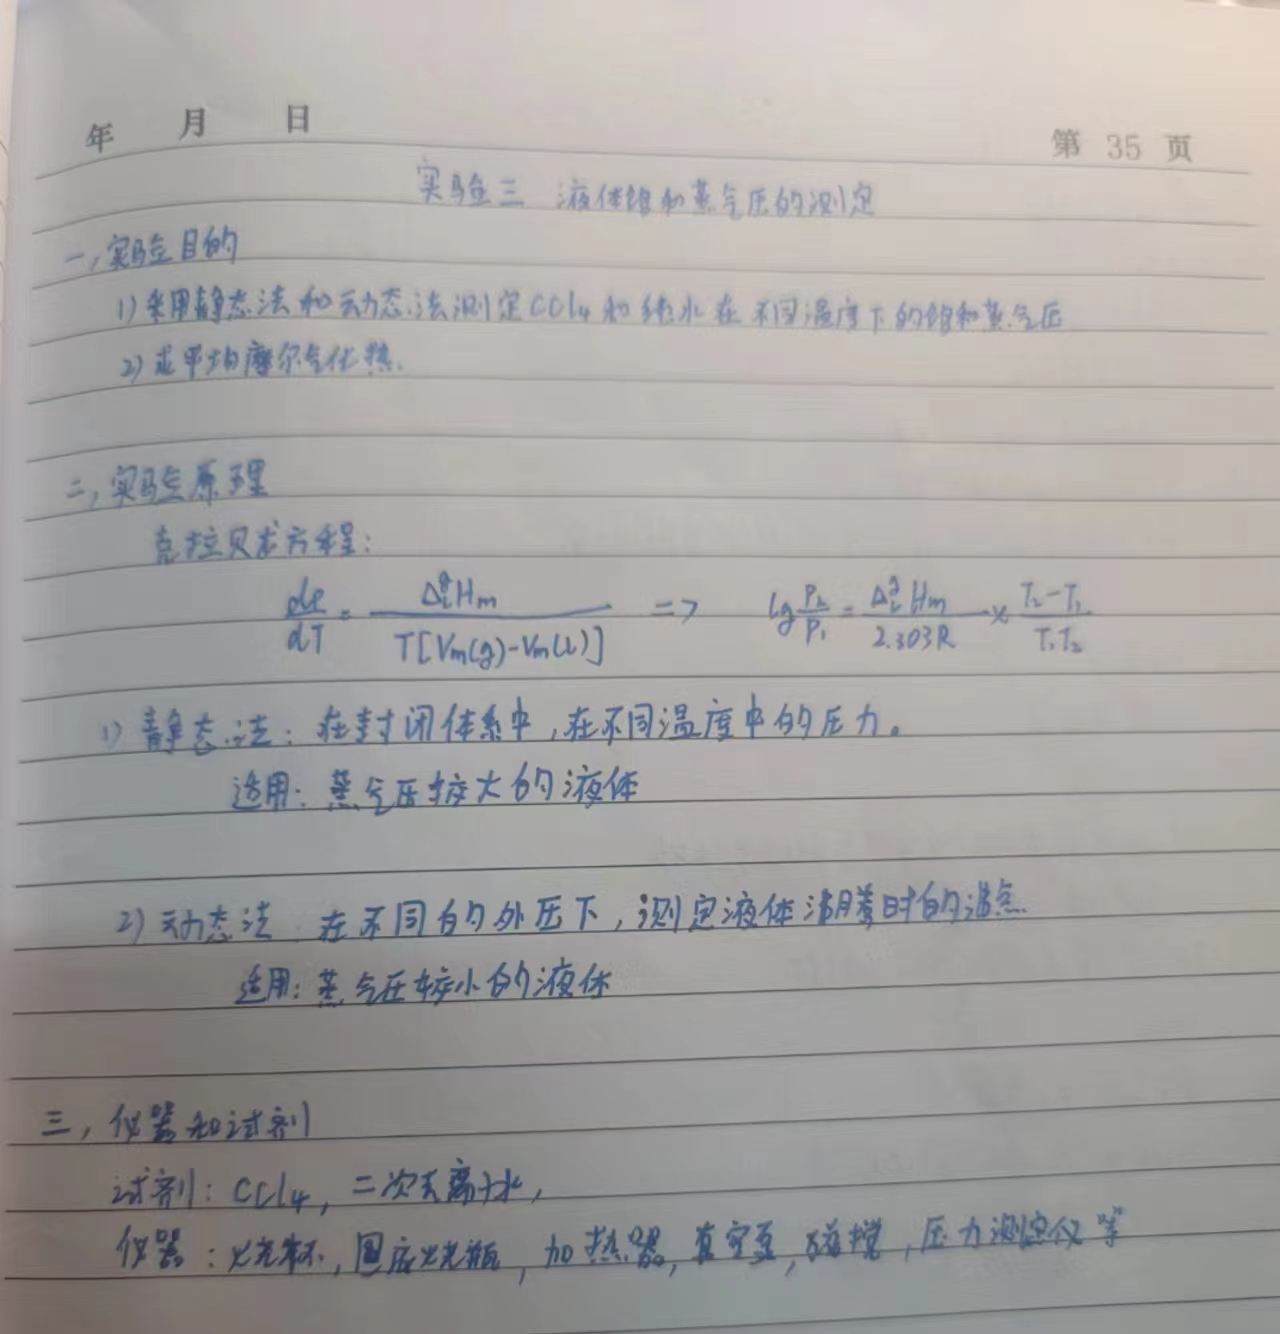
\includegraphics[width=0.8\textwidth]{1.png}
			\bicaption{实验预习报告的实验原理部分}{The principle part of the experiment in the experiment preview report}
		\end{figure}
			
	     
    \section{实验部分}
    	\subsection{仪器和试剂}
			试剂:\ \ $\rm CCl_{4}$,二次去离子水,$1000\ \ {\rm mL}$烧杯,$250\ \ {\rm mL}$两口圆底烧瓶等。\par 
			仪器:\ \ $\rm WXI-04$型数字式温度-压力测定仪,$\rm SHB-III$型循环水泵,电加热器,带电热套的磁力搅拌装置,冷凝水循环系统,真空缓冲罐,直形冷凝管,搅拌磁子,真空脂。
    			
    	 \subsection{实验内容}
		 本实验的实验操作如下所示,其中笔者的思考和具体实验中的不同操作会在括号中写出。\par
		 \subsubsection{动态法测$\rm H_{2}O$饱和蒸气压}
		 \textbf{1.组装仪器与气密性检验:}组装测量系统。将装有约$200\ \ {\rm mL}$去离子水和搅拌磁子的两口圆底烧瓶置于电加热套上并与冷凝管相连接。将温度探头通过橡皮塞插入烧瓶的侧口,探头尖端位于液面上侧,磨口处涂抹真空脂以防止漏气(具体实验装置如\textbf{图2}右侧所示)。打开回流冷凝水,调节流量适中。旋转储气罐阀门使系统与大气相通。打开公用循环真空泵,旋转储气罐阀门,使系统与大气隔绝、与真空泵相通,使压力计示数降至$49.89\ \ {\rm kPa}$;关闭活塞使系统与真空泵隔绝,$5\ \ {\rm min}$后压力计示数为$49.91\ \ {\rm kPa}$,变化小于$0.20\ \ {\rm kPa}$,表明体系气密性符合要求。\par
			 \begin{figure}[h]
				\centering
				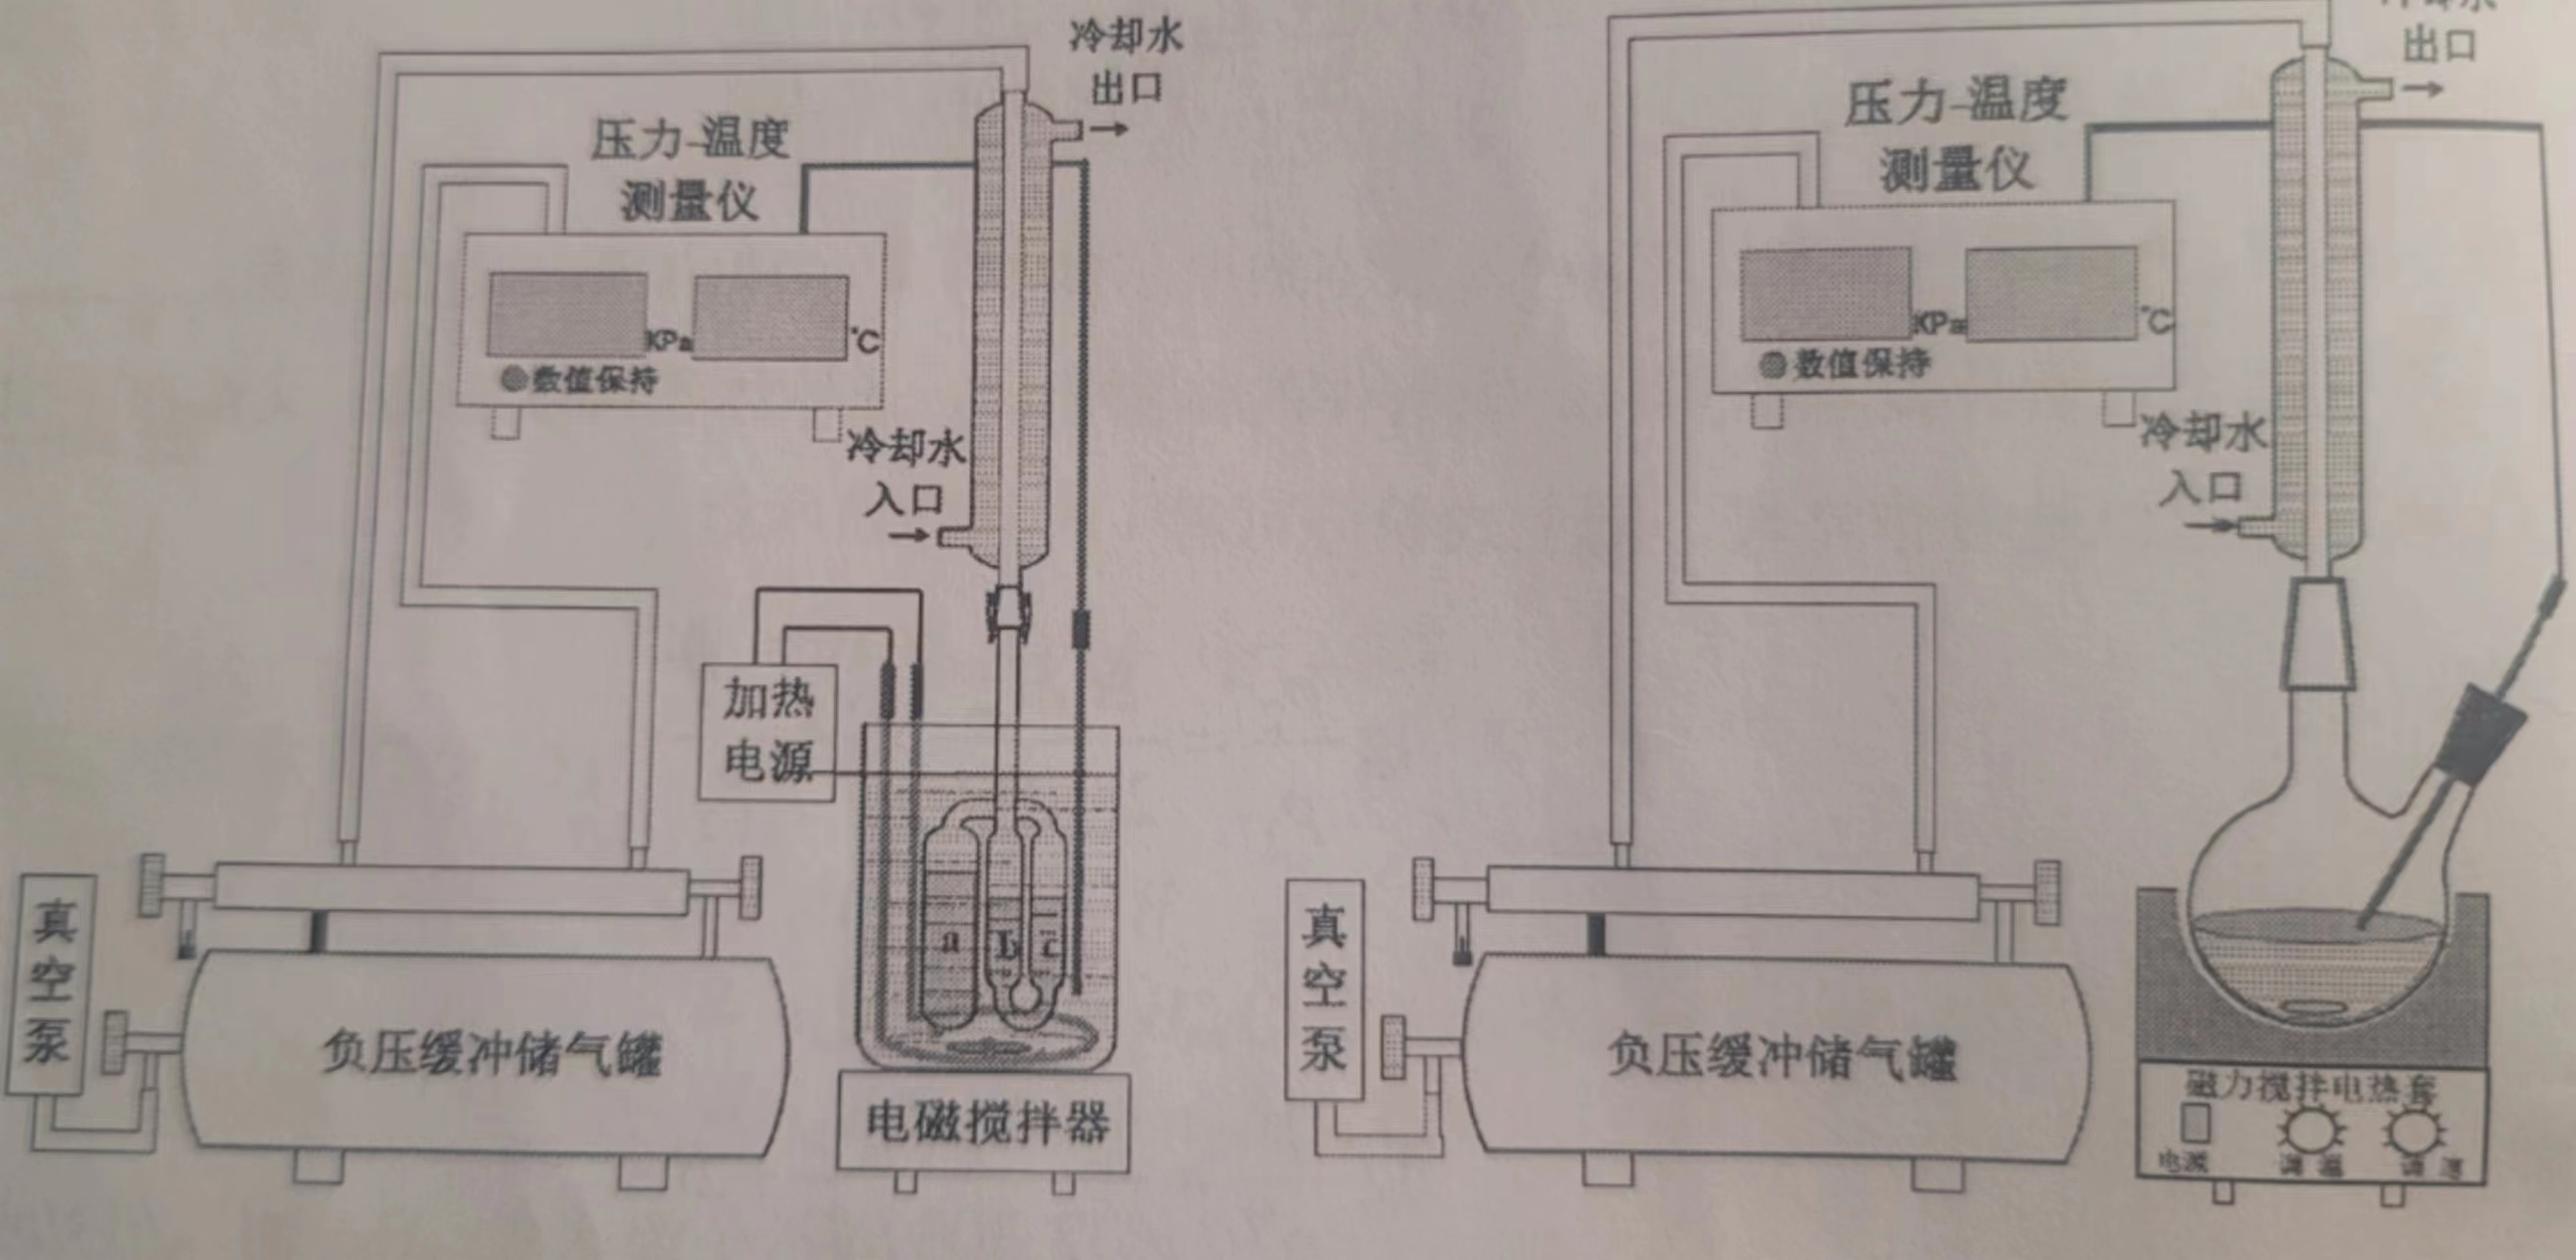
\includegraphics[width=0.9\textwidth]{2.png}
				\bicaption{动态发与静态法实验装置}{Dynamic and static experimental apparatus}
			\end{figure}
			\textbf{2.测量$\rm H_{2}O$不同温度的饱和蒸气压:}保持压差值为$\sim 50\ \ {\rm kPa}$,开始加热,不断搅拌。待烧瓶中水沸腾、温度计示数不再上升时,使用软件提供的Hold功能记录温度$t_{b}$和压力计示数$p_{b}$。停止加热,略微开启缓冲罐通大气的阀门,使少量空气进入系统,使内外压差降低$\sim 5\ \ {\rm kPa}$,关闭活塞,重新加热至沸腾,记录$t_{b}$和$p_{b}$。重复上述步骤,直至系统与大气完全相通。继续加热,测量$\rm H_{2}O$大气压下的沸点。平行测量3次,每次等体系温度略微冷却、水不再沸腾后重新加热至沸腾后测量。\textbf{(在之际过程中,因为圆底烧瓶和回流管会形成一个介稳系统,因此在温度在达到平台期后也会存在缓慢的上升,约0.005K/min,因此在实际实验过程中当温度30s没有明显变化就认为体系以达到平衡。)}\par 
			实验结束后,读取实验室内的大气压$p_{0}=102.68\ \ {\rm kPa}$,取实验前后大气压的平均值$p_{0}=103.07\ \ {\rm kPa}$作为实验过程中的大气压值。
		 \subsubsection{静态法测$\rm CCl_{4}$饱和蒸气压}
		 实验开始前,读取实验室内的大气压$p_{0}=102.81\ \ {\rm kPa}$,温度$t=18.7\ \ {\rm ^{\circ}C}$。\par
		 \textbf{1.排气与$\rm CCl_{4}$沸点测定:}利用前一组同学已验证气密性的测量系统直接进行实验(具体实验装置如\textbf{图2}左侧所示)。测$\rm CCl_{4}$大气压下的沸点。使体系与大气相通,水浴加热至$\sim 80\ \ {\rm ^{\circ}C}$,平衡管中有气泡产生,将平衡管中的空气排净。停止加热,不断搅拌,温度下降至一定程度时,$b$管中气泡开始消失,$c$管液面开始上升,同时$b$管液面下降。两管液面达到同一水平时,立即记下此时的温度计示数$t_{b}$和压力计示数$p_{b}$,重复赶气,平行测量多次$\rm CCl_{4}$大气压下的沸点,直至结果一致\textbf{(在实际实验过程中,因为开始加热和体系升温存在一个时间差。因此在b,c管液面即将持平时就应当打开加热,不然随着温度的下降,c管压力持续下降会引起空气的倒灌)}。\par 
		 \textbf{2.测量$\rm CCl_{4}$不同温度的饱和蒸气压:}立即关闭储气罐通向大气的活塞\textbf{(很重要,不然会发生空气的倒灌)},打开通真空泵的阀,使体系减压$\sim 5\ \ {\rm kPa}$,液体重又沸腾。关闭通真空泵的阀,不断搅拌,冷却至$b$、$c$两管液面等高时,记录温度$t_{b}$和压力计示数$p_{b}$。继续实验,每次减压$\sim 5\ \ {\rm kPa}$,直至压差值为$\sim 50\ \ {\rm kPa}$时,停止实验。\par
		\subsubsection{探究静态法中平衡管上端露出水浴时的影响}
			将平衡管上端露出水浴,并重复\textbf{2.2.2}中的步骤,先测量此时$\rm CCl_{4}$的沸点数据。关闭储气罐通向大气的活塞,打开通真空泵的阀,使体系减压$\sim 5\ \ {\rm kPa}$,液体重又沸腾。关闭通真空泵的阀,不断搅拌,冷却至$b$、$c$两管液面等高时,记录温度$t_{b}$和压力计示数$p_{b}$。继续实验,每次减压$\sim 5\ \ {\rm kPa}$,直至压差值为$\sim 80\ \ {\rm kPa}$时,停止实验。\par
			
	
	 \section{数据与结果}
 		\subsection{实验数据记录与处理}
		 	\subsubsection{测定$\rm H_{2}O$大气压下的沸点}
			 使用动态法测定$\rm H_{2}O$大气压下的沸点,平行测量3组数据,结果如\textbf{表1}所示\par
			 \begin{table}[h]
				\centering
				\zihao{5}
				\bicaption{$\rm H_{2}O$常压沸点测定实验数据}{$\rm H_{2}O$ Boiling Point Measurement Data at Normal Pressure}
				\begin{tabular}{ccccc}
					\toprule
					编号 & $p_{b}/{\rm kPa}$& $t_{b}/{\rm ^{\circ}C}$ \\
					\midrule
					1 & 102.69 & 99.25\\
					2 & 102.68 & 99.25\\
					3 & 102.68 & 99.26\\
					\bottomrule
				\end{tabular}
			\end{table}
			\par
			计算$\rm H_{2}O$常压沸点的平均值:
			$$
				\overline{t_{b}}=\frac{1}{3}\sum_{i=1}^{3}t_{b,i}=99.25\ \ {\rm ^{\circ}C}= 372.40\ \ {\rm K}
			$$
			常压沸点$t_{b}$的不确定度:
			$$
				u(t_{b})=\sqrt{\frac{1}{3-1}\sum_{i=1}^{3}(t_{b,i}-\overline{t_{b}})^{2}}=0.005\ \ {\rm K}
			$$
			故测得$\rm H_{2}O$常压沸点为:
			$$
				t_{b}=(372.40\pm 0.005)\ \ {\rm K}
			$$
			\par
 			\subsubsection{动态法测$\rm H_{2}O$饱和蒸气压}
			按照\textbf{2.2.1}中的是步骤测量水不同温度下的饱和蒸汽压,结果如\textbf{表2}所示。
			\begin{table}[h]
				\centering
				\zihao{5}
				\bicaption{动态法测$\rm H_{2}O$沸点实验数据}{$\rm H_{2}O$ Boiling Point Measurement Data by Dynamic Method}
				\begin{tabular}{ccccccc}
					\toprule
					编号 & $t_{b}/{\rm ^{\circ}C}$& $p_{b}/{\rm kPa}$ &&编号 & $t_{b}/{\rm ^{\circ}C}$ & $p_{b}/{\rm kPa}$  \\
					\midrule
					1  & 80.46 & 50.99 &&7& 92.69 & 80.28\\
					2  & 83.29 & 56.30 &&8& 94.19 & 85.22 \\
					3  & 85.04 & 60.14 &&9& 95.64 & 90.03\\
					4  & 87.09 & 65.35 &&10& 97.20 & 95.28  \\
					5  & 89.15 & 70.61 &&11& 98.27 & 99.05 \\
					6  & 90.92 & 75.41 &&12& 99.25 & 102.68 \\
					\bottomrule
				\end{tabular}
			\end{table}
		\subsubsection{静态法测$\rm CCl_{4}$常压沸点}
		使用静态法测定$\rm CCl_{4}$大气压下的沸点,平行测量3组数据,结果如\textbf{表3}所示\par
		\begin{table}[h]
			\centering
			\zihao{5}
			\bicaption{$\rm CCl_{4}$常压沸点测定实验数据}{$\rm CCl_{4}$ Boiling Point Measurement Data at Normal Pressure}
			\begin{tabular}{ccccc}
				\toprule
				编号 & $p_{b}/{\rm kPa}$& $t_{b}/{\rm ^{\circ}C}$ \\
				\midrule
				1 & 102.81 & 76.89\\
				2 & 102.81 & 76.93\\
				3 & 102.83 & 76.86\\
				\bottomrule
			\end{tabular}
		\end{table}
		\par
		三组数据的平行性较好,说明平衡管内的空气已经排净,可以进行后续实验。\par
		计算$\rm CCl_{4}$常压沸点的平均值:
		$$
			\overline{t_{b}}=\frac{1}{3}\sum_{i=1}^{3}t_{b,i}=76.89\ \ {\rm ^{\circ}C}= 350.04\ \ {\rm K}
		$$
		常压沸点$t_{b}$的不确定度:
		$$
			u(t_{b})=\sqrt{\frac{1}{3-1}\sum_{i=1}^{3}(t_{b,i}-\overline{t_{b}})^{2}}=0.03\ \ {\rm K}
		$$
		故测得$\rm CCl_{4}$常压沸点为:
		$$
			t_{b}=(350.04\pm 0.03)\ \ {\rm K}
		$$
		\par
		\subsubsection{静态法测$\rm CCl_{4}$饱和蒸气压}
		按照\textbf{2.2.2}中的是步骤测量$\rm CCl_{4}$不同温度下的饱和蒸汽压,结果如\textbf{表4}所示。
		\begin{table}[h]
			\centering
			\zihao{5}
			\bicaption{静态法测$\rm CCl_{4}$沸点实验数据}{$\rm CCl_{4}$ Boiling Point Measurement Data by Static Method}
			\begin{tabular}{ccccccc}
				\toprule
				编号 & $t_{b}/{\rm ^{\circ}C}$& $p_{b}/{\rm kPa}$ &&编号 & $t_{b}/{\rm ^{\circ}C}$ & $p_{b}/{\rm kPa}$  \\
				\midrule
				1  & 76.89 & 102.81 &&7& 64.83 & 69.97\\
				2  & 74.40 & 95.29 &&8& 62.42 & 64.66 \\
				3  & 72.38 & 89.54 &&9& 60.33 & 60.28\\
				4  & 70.87 & 85.54 &&10& 58.02 & 55.67  \\
				5  & 69.00 & 80.34 &&11& 55.04 & 50.21 \\
				6  & 67.32 & 75.93 &&&& \\
				\bottomrule
			\end{tabular}
		\end{table}
		\par
	\subsection{数据处理结果与分析}
		\subsubsection{动态法测$\rm H_{2}O$饱和蒸气压}
		由\textbf{3.1.2}中可得动态法测$\rm H_{2}O$沸点实验数据,利用$T=t_{b}+273.15\ \ {\rm K}$将$\rm H_{2}O$的沸点$t_{b}$转化为热力学温标$T$,取标准大气压$p^{\ominus}=100.0\ \ {\rm kPa}$,计算${\rm ln}(p/p^{\ominus})$和$T^{-1}$,结果如\textbf{表5}所示:
		\begin{table}[h]
			\centering
			\zihao{5}
			\bicaption{$\rm H_{2}O$ $p-T$关系相关计算数据}{$\rm H_{2}O$ $p-T$ Relationship Calculation Data}
			\begin{tabular}{cccccc}
				\toprule
				编号 & $t_{b}/{\rm ^{\circ}C}$& $T/{\rm K}$ & $p/{\rm kPa}$ & ${\rm ln}(p/p^{\ominus})$ & $T^{-1}/{\rm 10^{-3}\ \ K^{-1}}$\\
				\midrule
				1  & 80.46 & 353.61 & 50.99  & -0.6735 & 2.8280 \\
				2  & 83.29 & 356.44 & 56.3   & -0.5745 & 2.8055 \\
				3  & 85.04 & 358.19 & 60.14  & -0.5085 & 2.7918   \\
				4  & 87.09 & 360.24 & 65.35  & -0.4254 & 2.7759  \\
				5  & 89.15 & 362.3  & 70.61  & -0.3480 & 2.7601 \\
				6  & 90.92 & 364.07 & 75.41  & -0.2822& 2.7467 \\
				7  & 92.6  & 365.75 & 80.28  & -0.2196 & 2.734 \\
				8  & 94.19 & 367.34 & 85.22  & -0.1599 & 2.722 \\
				9  & 95.64 & 368.79 & 90.03  & -0.1050& 2.7116  \\
				10 & 97.2  & 370.35 & 95.28  & -0.0483 & 2.7001 \\
				11 & 98.26 & 371.41 & 99.06  & -0.0094& 2.6924\\
				12 & 99.25 & 372.4  & 102.68 & 0.0264  & 2.6853  \\
				\bottomrule
			\end{tabular}
		\end{table}
		\par
		根据\textbf{表5}数据,作出$p-T$关系的散点图,使用origin提供的b样条将各散点链接,结果如\textbf{图3}所示:
		\begin{figure}[!h]
			\centering
			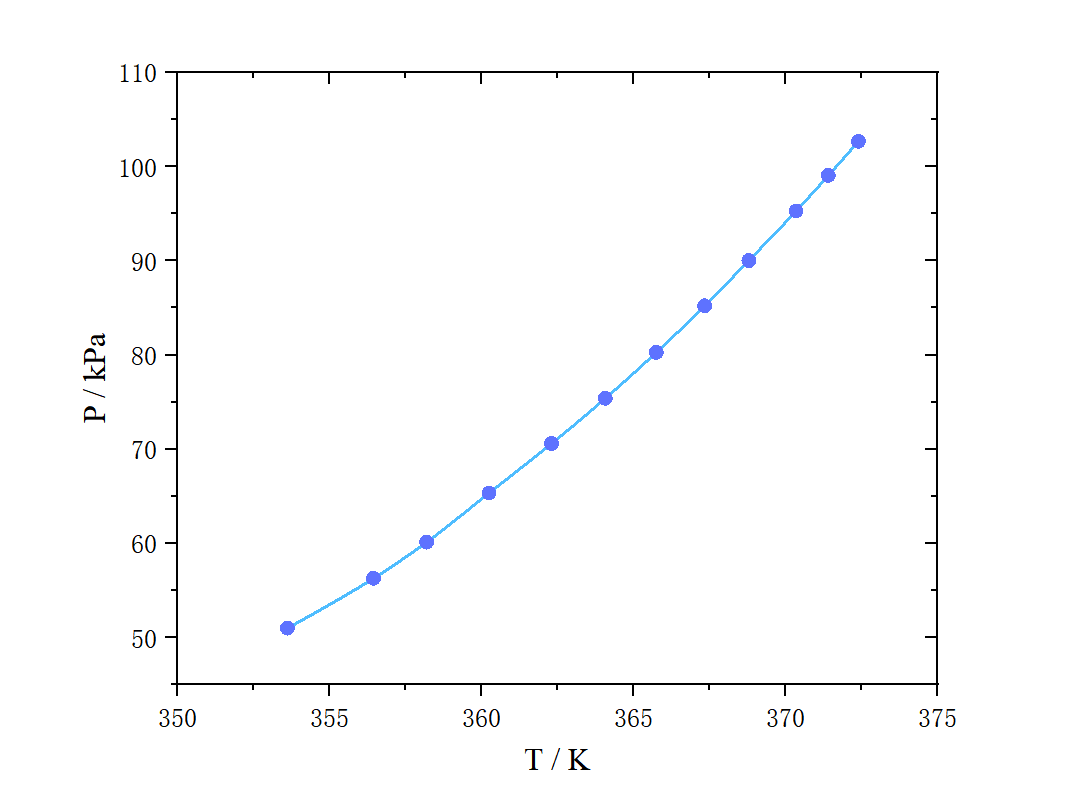
\includegraphics[width=0.7\textwidth]{3.png}
			\bicaption{$\rm H_{2}O$ $p-T$关系图}{$\rm H_{2}O$ $p-T$ Relationship Graph}
		\end{figure}
		\par
		根据\textbf{表5}数据,作出${\rm ln}(p/p^{\ominus})$-$T^{-1}$关系的散点图,并对其进行线性拟合,作出拟合直线,如\textbf{图4}所示:
		\begin{figure}[!h]
			\centering
			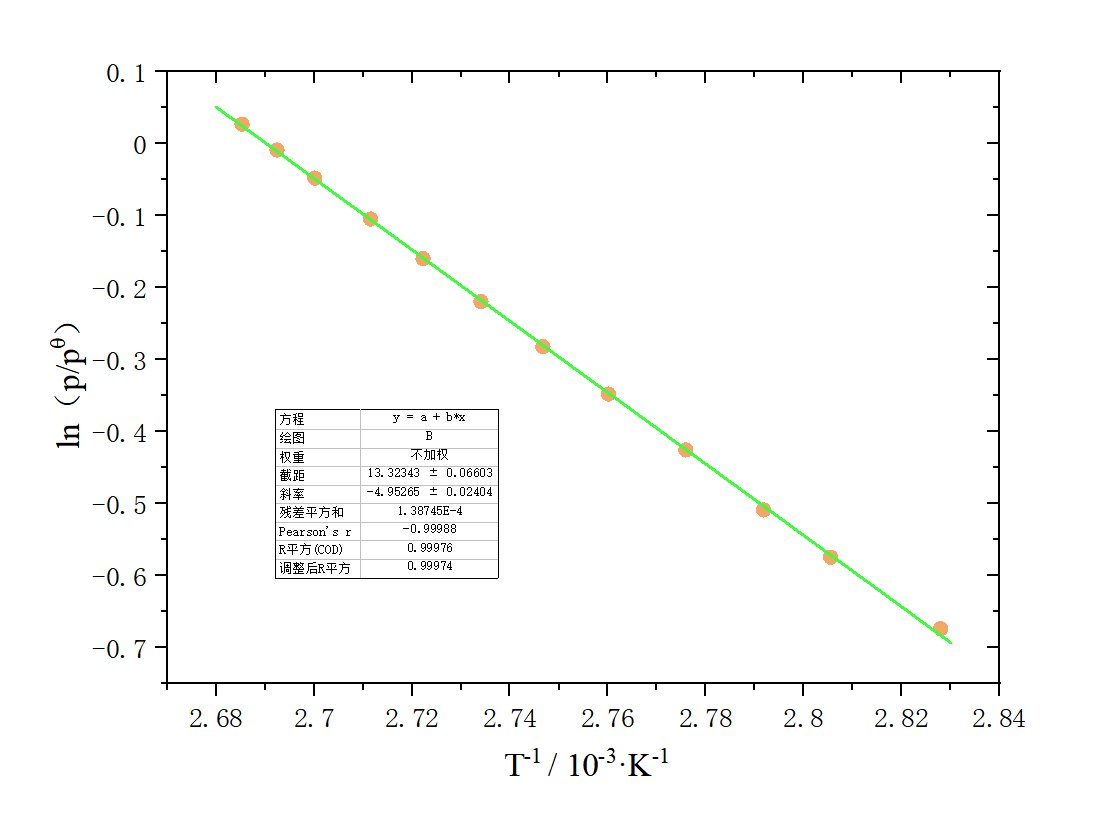
\includegraphics[width=0.7\textwidth]{4.png}
			\bicaption{$\rm H_{2}O$ ${\rm ln}(p/p^{\ominus})$-$T^{-1}$关系图}{$\rm H_{2}O$ ${\rm ln}(p/p^{\ominus})$-$T^{-1}$ Relationship Graph}
		\end{figure}
		\par
		拟合直线的方程为:
		$$
			{\rm ln}(p/p^{\ominus})=(-4952.65\pm 24)\cdot T^{-1}+(13.323 \pm 0.066) \ \ \ \ R^{2}=0.9997
		$$
		\par
		$|R|\approx 1$,可见${\rm ln}(p/p^{\ominus})$-$T^{-1}$具有很好的线性关系,与Clausius-Clapeyron方程相符。根据\textbf{图4}中${\rm ln}(p/p^{\ominus})$-$T^{-1}$拟合直线的方程,代入$p=1\ \ {\rm atm}=101.3\ \ {\rm kPa}$,计算$\rm H_{2}O$的沸点:\par 
		$$
			T_{b}=\frac{4952.65}{(13.323-{\rm ln}(101.3/100.0))}=372.11\ \ {\rm K}
		$$
		\par
		查阅\textit{CRC Handbook of Chemistry and Physics}\citealp{crc},知$\rm H_{2}O$在$\rm 1\ \ atm$下的沸点$t_{b}=100.0\ \ {\rm ^{\circ}C}$,实验计算结果与参考值相近。\par 
		计算$\rm H_{2}O$的平均摩尔气化热$\Delta^{\rm g}_{\rm l}H_{m}$。根据拟合直线斜率大小A,可知:
		$$
			\Delta^{\rm g}_{\rm l}H_{m}=-A\cdot R=41.18\ \ {\rm kJ\cdot mol^{-1}}
		$$
		$\Delta^{\rm g}_{\rm l}H_{m}$的不确定度:
		$$
			u(\Delta^{\rm g}_{\rm l}H_{m})=u(A)\cdot R=0.20\ \ {\rm kJ\cdot mol^{-1}}
		$$
		故测得$\rm H_{2}O$的平均摩尔气化热为:
		$$
			\Delta^{\rm g}_{\rm l}H_{m}=(41.18\pm 0.20)\ \ {\rm kJ\cdot mol^{-1}}
		$$
		\par
		查阅\textit{CRC Handbook of Chemistry and Physics}\citealp{crc},知$\rm H_{2}O$在常压沸点下$\Delta^{\rm g}_{\rm l}H_{m}=40.65\ \ {\rm kJ\cdot mol^{-1}}$,实验计算结果与参考值相当接近。
		计算$\rm H_{2}O$的摩尔气化熵$\Delta^{\rm g}_{\rm l}S_{m}$。
		根据\textbf{3.1.1},实验测得$\rm H_{2}O$常压沸点:
		$$
			t_{b}=(372.40\pm 0.005)\ \ {\rm K}
		$$
		在常压沸点$t_{b}$下,自由能变$\Delta^{\rm g}_{\rm l}G_{m}=0$,故
		$$
			\Delta^{\rm g}_{\rm l}S_{m}=\frac{\Delta^{\rm g}_{\rm l}H_{m}}{t_{b}}=110.6\ \ {\rm J\cdot K^{-1}\cdot mol^{-1}}
		$$
		$\Delta^{\rm g}_{\rm l}S_{m}$的不确定度为:
		$$
			u(\Delta^{\rm g}_{\rm l}S_{m})=\frac{1}{T_{b}} \sqrt{\sigma^{2}_{\Delta^{\rm g}_{\rm l}H_{m}}+\frac{\Delta^{\rm g}_{\rm l}H_{m}^{2}}{T_{b}^{2}}\sigma^{2}_{t_{b}}}=0.2\ \ {\rm J\cdot K^{-1}\cdot mol^{-1}}
		$$
		故测得$\rm H_{2}O$的摩尔气化熵为:
		$$
			\Delta^{\rm g}_{\rm l}S_{m}=(110.6\pm 0.2)\ \ {\rm J\cdot K^{-1}\cdot mol^{-1}}
		$$
		\par
		根据Trouton规则,在常压沸点下各正常液体的摩尔气化熵相同,为$\Delta S\approx 88\ \ {\rm J\cdot K^{-1}\cdot mol^{-1}}$。实验得到$\rm H_{2}O$摩尔气化熵的计算结果与Trouton规则偏差较大,远大于$88\ \ {\rm J\cdot K^{-1}\cdot mol^{-1}}$。分析可能的原因是液态水中存在大量分子间氢键,在气化过程中需克服氢键相互作用,带来了额外的熵效应,故水的摩尔气化熵明显$>88\ \ {\rm J\cdot K^{-1}\cdot mol^{-1}}$,偏离Trouton规则。
		\par
		\subsubsection{静态法测$\rm CCl_{4}$饱和蒸气压}
		由\textbf{3.1.4}中可得静态法测$\rm CCl_{4}$沸点实验数据,利用$T=t_{b}+273.15\ \ {\rm K}$将$\rm CCl_{4}$的沸点$t_{b}$转化为热力学温标$T$,取标准大气压$p^{\ominus}=100.0\ \ {\rm kPa}$,计算${\rm ln}(p/p^{\ominus})$和$T^{-1}$,结果如\textbf{表6}所示:
		\begin{table}[h]
			\centering
			\zihao{5}
			\bicaption{$\rm CCl_{4}$ $p-T$关系相关计算数据}{$\rm CCl_{4}$ $p-T$ Relationship Calculation Data}
			\begin{tabular}{cccccc}
				\toprule
				编号 & $t_{b}/{\rm ^{\circ}C}$& $T/{\rm K}$ & $p/{\rm kPa}$ & ${\rm ln}(p/p^{\ominus})$ & $T^{-1}/{\rm 10^{-3}\ \ K^{-1}}$\\
				\midrule
				1  & 76.86 & 350.01 & 102.83 & 0.0279  & 2.8571 \\
				2  & 74.40 & 347.55 & 95.29  & -0.0482 & 2.8773 \\
				3  & 72.38 & 345.53 & 89.54  & -0.1105 & 2.8941 \\
				4  & 70.87 & 344.02 & 85.54  & -0.1562 & 2.9068 \\
				5  & 69.00 & 342.15 & 80.34  & -0.2189 & 2.9227 \\
				6  & 67.32 & 340.47 & 75.93  & -0.2754 & 2.9371 \\
				7  & 64.83 & 337.98 & 69.97  & -0.3571 & 2.9588 \\
				8  & 62.42 & 335.57 & 64.66  & -0.4360 & 2.9800 \\
				9  & 60.33 & 333.48 & 60.28  & -0.5062 & 2.9987 \\
				10 & 58.02 & 331.17 & 55.67  & -0.5857 & 3.0196 \\
				11 & 55.04 & 328.19 & 50.21  & -0.6890 & 3.0470 \\
				\bottomrule
			\end{tabular}
		\end{table}
		\par
		根据\textbf{表6}数据,作出$p-T$关系的散点图,使用origin提供的b样条将各散点链接,结果如\textbf{图5}所示:
		\begin{figure}[!h]
			\centering
			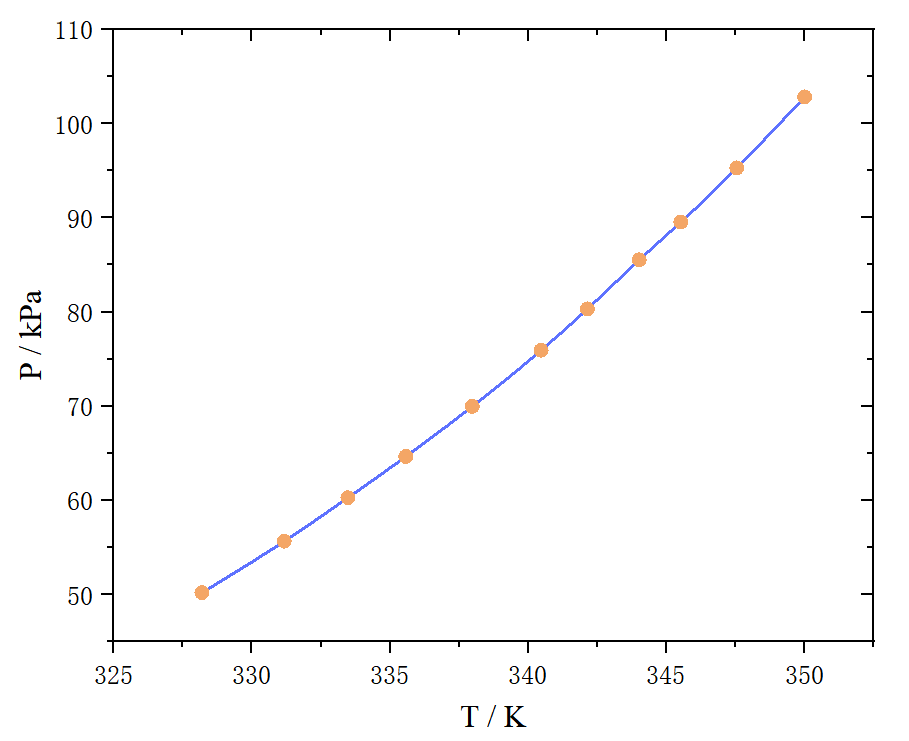
\includegraphics[width=0.65\textwidth]{5.png}
			\bicaption{$\rm CCl_{4}$ $p-T$关系图}{$\rm CCl_{4}$ $p-T$ Relationship Graph}
		\end{figure}
		\par
		根据\textbf{表6}数据,作出${\rm ln}(p/p^{\ominus})$-$T^{-1}$关系的散点图,并对其进行线性拟合,作出拟合直线,如\textbf{图6}所示:
		\begin{figure}[!h]
			\centering
			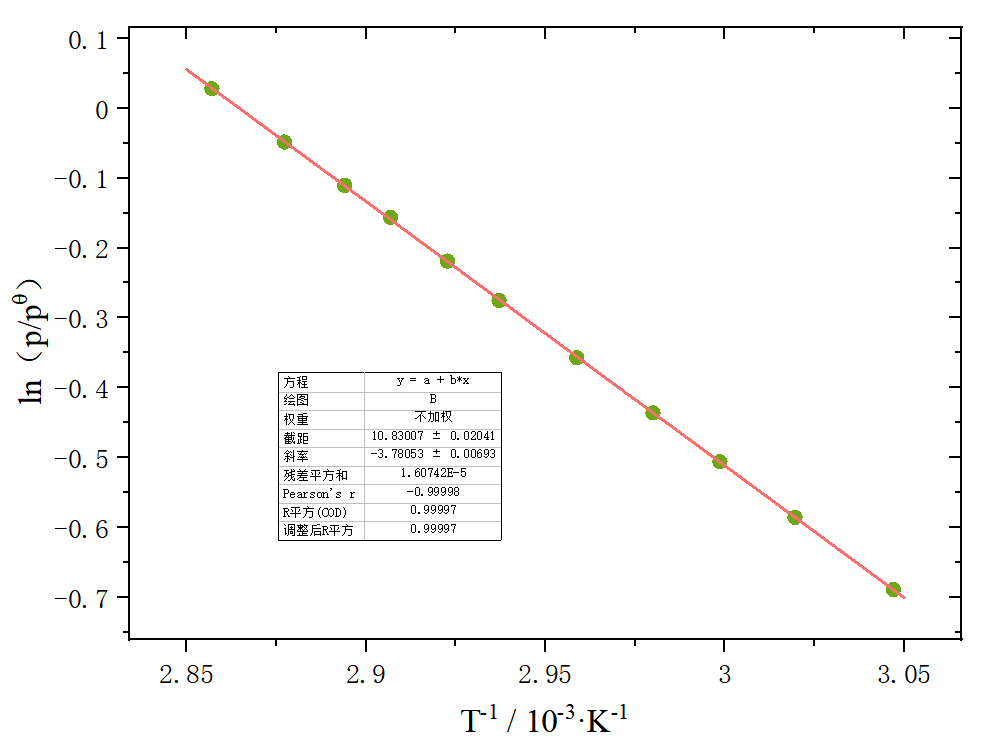
\includegraphics[width=0.65\textwidth]{6.png}
			\bicaption{$\rm CCl_{4}$ ${\rm ln}(p/p^{\ominus})$-$T^{-1}$关系图}{$\rm CCl_{4}$ ${\rm ln}(p/p^{\ominus})$-$T^{-1}$ Relationship Graph}
		\end{figure}
		\par
		拟合直线的方程为:
		$$
			{\rm ln}(p/p^{\ominus})=(-3780.53\pm 6.90)\cdot T^{-1}+(10.83 \pm 0.02) \ \ \ \ R^{2}=0.99997
		$$
		\par
		$|R|\approx 1$,可见${\rm ln}(p/p^{\ominus})$-$T^{-1}$具有很好的线性关系,与Clausius-Clapeyron方程相符。根据\textbf{图6}中${\rm ln}(p/p^{\ominus})$-$T^{-1}$拟合直线的方程,代入$p=1\ \ {\rm atm}=101.3\ \ {\rm kPa}$,计算$\rm CCl_{4}$的沸点:\par
		$$
			T_{b}=\frac{3780.53}{(10.83-{\rm ln}(101.3/100.0))}=349.50\ \ {\rm K}
		$$
		\par
		查阅\textit{CRC Handbook of Chemistry and Physics}\citealp{crc},知$\rm CCl_{4}$在$\rm 1\ \ atm$下的沸点$t_{b}=76.72\ \ {\rm ^{\circ}C}$,实验计算结果与参考值相近。\par
		计算$\rm CCl_{4}$的平均摩尔气化热$\Delta^{\rm g}_{\rm l}H_{m}$。根据拟合直线斜率大小A,可知:
		$$
			\Delta^{\rm g}_{\rm l}H_{m}=-A\cdot R=31.43\ \ {\rm kJ\cdot mol^{-1}}
		$$
		$\Delta^{\rm g}_{\rm l}H_{m}$的不确定度:
		$$
			u(\Delta^{\rm g}_{\rm l}H_{m})=u(A)\cdot R=0.08\ \ {\rm kJ\cdot mol^{-1}}
		$$
		故测得$\rm CCl_{4}$的平均摩尔气化热为:
		$$
			\Delta^{\rm g}_{\rm l}H_{m}=(31.43\pm 0.08)\ \ {\rm kJ\cdot mol^{-1}}
		$$
		\par
		查阅\textit{CRC Handbook of Chemistry and Physics}\citealp{crc},知$\rm CCl_{4}$在常压沸点下$\Delta^{\rm g}_{\rm l}H_{m}=29.82\ \ {\rm kJ\cdot mol^{-1}}$,实验计算结果与参考值有一定的偏差。
		计算$\rm CCl_{4}$的摩尔气化熵$\Delta^{\rm g}_{\rm l}S_{m}$。
		根据\textbf{3.1.3},实验测得$\rm CCl_{4}$常压沸点:
		$$
			t_{b}=(350.04\pm 0.03)\ \ {\rm K}
		$$
		在常压沸点$t_{b}$下,自由能变$\Delta^{\rm g}_{\rm l}G_{m}=0$,故
		$$
			\Delta^{\rm g}_{\rm l}S_{m}=\frac{\Delta^{\rm g}_{\rm l}H_{m}}{t_{b}}=89.1\ \ {\rm J\cdot K^{-1}\cdot mol^{-1}}
		$$
		$\Delta^{\rm g}_{\rm l}S_{m}$的不确定度为:
		$$
			u(\Delta^{\rm g}_{\rm l}S_{m})=\frac{1}{T_{b}} \sqrt{\sigma^{2}_{\Delta^{\rm g}_{\rm l}H_{m}}+\frac{\Delta^{\rm g}_{\rm l}H_{m}^{2}}{T_{b}^{2}}\sigma^{2}_{t_{b}}}=0.22\ \ {\rm J\cdot K^{-1}\cdot mol^{-1}}
		$$
		故测得$\rm CCl_{4}$的摩尔气化熵为:
		$$
			\Delta^{\rm g}_{\rm l}S_{m}=(89.1\pm 0.22)\ \ {\rm J\cdot K^{-1}\cdot mol^{-1}}
		$$
		\par
		根据Trouton规则,在常压沸点下各正常液体的摩尔气化熵相同,为$\Delta S\approx 88\ \ {\rm J\cdot K^{-1}\cdot mol^{-1}}$。实验得到$\rm CCl_{4}$摩尔气化熵的计算结果与Trouton规则基本相同,为$89.1\ \ {\rm J\cdot K^{-1}\cdot mol^{-1}}$,与Trouton规则吻合。

 	\section{讨论与结论}
	 \subsection{误差与误差分析}
		\subsubsection{实验误差}
		本实验使用动态法测定$\rm H_{2}O$的平均摩尔气化热$\Delta^{\rm g}_{\rm l}H_{m}=(41.18\pm 0.20)\ \ {\rm kJ\cdot mol^{-1}}$,对比文献参考值\citealp{crc}$\Delta^{\rm g}_{\rm l}H_{m}=40.65\ \ {\rm kJ\cdot mol^{-1}}$,实验测定值略大于文献参考值,结果的相对误差:
		$$
			\delta_{\Delta^{\rm g}_{\rm l}H_{m}}=\frac{41.18-40.65}{40.65}\times 100\% =1.3\%
		$$
		\par
		可知测定结果的相对误差在可接受范围内,$\Delta^{\rm g}_{\rm l}H_{m}$测定相当准确。笔者认为动态法测$\Delta^{\rm g}_{\rm l}H_{m}$可能的误差来源可能包括:
		\begin{enumerate}
			\item \textbf{电热套的热辐射对温度计的影响}:实验中电热套的热辐射对温度计的影响,导致实验中温度计测量温度与$\rm H_{2}O$实际温度有一定偏差。
			\item \textbf{温度计位置有所偏差}:温度计放置位置一定程度上影响测定准确性,若温度计位置在液面以下,测得温度可能为未沸腾部分水的温度,为温度测量引入一定误差。
		\end{enumerate}
		\par
		本实验使用静态法测定$\rm CCl_{4}$的平均摩尔气化热$\Delta^{\rm g}_{\rm l}H_{m}=(31.43\pm 0.08)\ \ {\rm kJ\cdot mol^{-1}}$,对比文献参考值\citealp{crc}$\Delta^{\rm g}_{\rm l}H_{m}=29.82\ \ {\rm kJ\cdot mol^{-1}}$,实验测定值略大于文献参考值,结果的相对误差:
		$$
			\delta_{\Delta^{\rm g}_{\rm l}H_{m}}=\frac{31.43-29.82}{29.82}\times 100\% =5.4\%
		$$
		\par
		笔者认为静态法测$\Delta^{\rm g}_{\rm l}H_{m}$可能的误差来源可能包括:
		\begin{enumerate}
			\item \textbf{平衡管内空气可能未完全排净}:$c$两管液面上方仍存在少量空气,使得$\rm CCl_{4}$的饱和蒸气压与实际压强略有偏差。
			\item \textbf{水浴温度不能完全表示体系温度}:实验中温度计测量温度为水浴温度,而实验中温度变化较快,不能保证平衡管与水浴时刻保持热平衡,测得温度与$\rm CCl_{4}$实际温度有一定偏差。
		\end{enumerate}
		\par

		
		\subsection{探究实验}
		\subsubsection{静态法中平衡管上端露出水浴}
		在与同组同学交流的过程中,有同学提出了若将平衡管上端露出水浴,可能会引入一定的误差。为了探究这一问题,笔者进行了探究实验,实验结果如下:\par
		测量$\rm CCl_{4}$常压沸点:
		\begin{table}[h]
			\centering
			\zihao{5}
			\bicaption{平衡管上端露出水浴时$\rm CCl_{4}$常压沸点测定实验数据}{Measurement Data with the Upper End of the Equilibrium Tube Exposed to the Water Bath}
			\begin{tabular}{ccccc}
				\toprule
				编号 & $p_{b}/{\rm kPa}$& $t_{b}/{\rm ^{\circ}C}$ \\
				\midrule
				1 & 102.81 & 77.59\\
				2 & 102.81 & 77.72\\
				3 & 102.83 & 77.69\\
				\bottomrule
			\end{tabular}
		\end{table}
		\par
		计算$\rm CCl_{4}$常压沸点的平均值:
		$$
			\overline{t_{b}}=\frac{1}{3}\sum_{i=1}^{3}t_{b,i}=77.67\ \ {\rm ^{\circ}C}= 350.82\ \ {\rm K}
		$$
		常压沸点$t_{b}$的不确定度:
		$$
			u(t_{b})=\sqrt{\frac{1}{3-1}\sum_{i=1}^{3}(t_{b,i}-\overline{t_{b}})^{2}}=0.07\ \ {\rm K}
		$$
		相比于\textbf{3.1.3}中的实验结果,露出水浴后测得的$\rm CCl_{4}$常压沸点$t_{b}$略大于未露出水浴时测得的$t_{b}$,同时其不确定度也略大于未露出水浴时的不确定度。
		\par
		进一步测量不同温度下$\rm CCl_{4}$的饱和蒸气压,结果如下:
		\begin{table}[h]
			\centering
			\zihao{5}
			\bicaption{平衡管上端露出水浴时$\rm CCl_{4}$沸点实验数据}{Measurement Data with the Upper End of the Equilibrium Tube Exposed to the Water Bath}
			\begin{tabular}{cccccc}
				\toprule
				编号 & $t_{b}/{\rm ^{\circ}C}$& $T/{\rm K}$ & $p/{\rm kPa}$ & ${\rm ln}(p/p^{\ominus})$ & $T^{-1}/{\rm 10^{-3}\ \ K^{-1}}$\\
				\midrule
				1 & 77.69 & 350.84 & 102.8 & 0.027615167  & 2.850302132 \\
				2 & 75.13 & 348.28 & 95.37 & -0.047406122 & 2.871253015 \\
				3 & 72.71 & 345.86 & 88.52 & -0.121941671 & 2.891343318 \\
				4 & 71.39 & 344.54 & 84.57 & -0.167590592 & 2.902420619 \\
				5 & 69.65 & 342.8  & 80.41 & -0.218031639 & 2.917152859 \\
				\bottomrule
			\end{tabular}
		\end{table}
		\par
		根据\textbf{表8}数据,作出$p-T$关系的散点图,使用origin提供的b样条将各散点链接,结果如\textbf{图7}所示:
		\begin{figure}[!h]
			\centering
			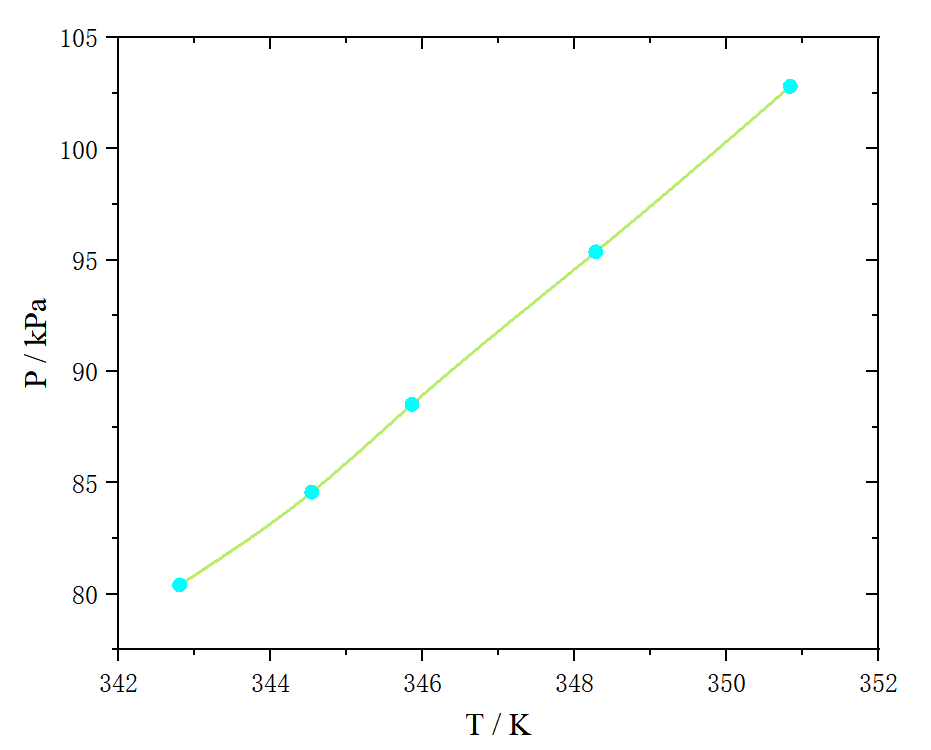
\includegraphics[width=0.65\textwidth]{7.png}
			\bicaption{平衡管上端露出水浴时$\rm CCl_{4}$ $p-T$关系图}{The $p-T$ with the Upper End of the Equilibrium Tube Exposed to the Water Bath}
		\end{figure}
		\par
		根据\textbf{表8}数据,作出${\rm ln}(p/p^{\ominus})$-$T^{-1}$关系的散点图,并对其进行线性拟合,作出拟合直线,如\textbf{图8}所示:
		\begin{figure}[!h]
			\centering
			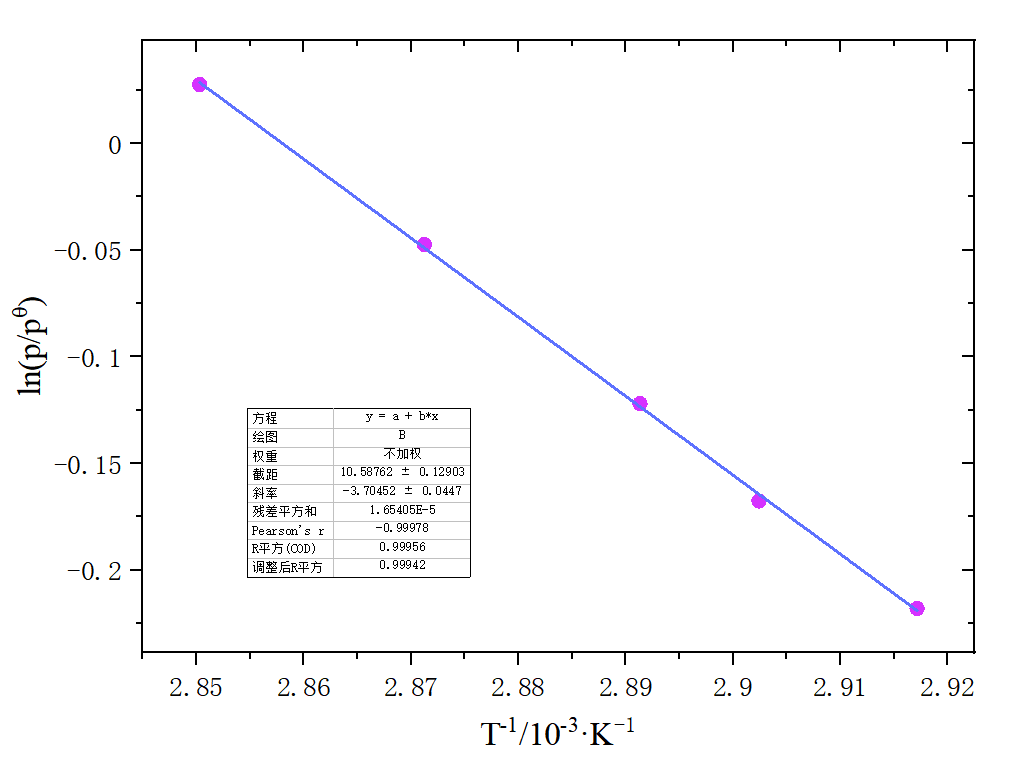
\includegraphics[width=0.65\textwidth]{8.png}
			\bicaption{平衡管上端露出水浴时$\rm CCl_{4}$ ${\rm ln}(p/p^{\ominus})$-$T^{-1}$关系图}{The ${\rm ln}(p/p^{\ominus})$-$T^{-1}$ with the Upper End of the Equilibrium Tube Exposed to the Water Bath}
		\end{figure}
		\par
		拟合直线的方程为:
		$$
			{\rm ln}(p/p^{\ominus})=(-3704.52\pm 44.70)\cdot T^{-1}+(10.59 \pm 0.129) \ \ \ \ R^{2}=0.9995
		$$
		\par
		尽管在此情况下,拟合直线的斜率和截距的误差均有所变大(约一个数量级),其$|R|\approx 1$,可见${\rm ln}(p/p^{\ominus})$-$T^{-1}$仍然具有很好的线性关系。根据\textbf{图8}中${\rm ln}(p/p^{\ominus})$-$T^{-1}$拟合直线的方程,代入$p=1\ \ {\rm atm}=101.3\ \ {\rm kPa}$,计算$\rm CCl_{4}$的沸点:\par
		$$
			T_{b}=\frac{3704.52}{(10.59-{\rm ln}(101.3/100.0))}=348.28\ \ {\rm K}
		$$
		\par
		查阅\textit{CRC Handbook of Chemistry and Physics}\citealp{crc},知$\rm CCl_{4}$在$\rm 1\ \ atm$下的沸点$t_{b}=76.72\ \ {\rm ^{\circ}C}$,其相对误差,$\delta_{t_{b}}$:
		$$
			\delta_{t_{b}}=\frac{348.28-349.87}{349.67}\times 100\%  = 0.45\%
		$$
		\par
		可见露出水浴后测得的$\rm CCl_{4}$沸点$t_{b}$与未露出水浴时测得的$t_{b}$相比,误差略有增大,但仍然在可接受范围内,露出水浴后测得的$\rm CCl_{4}$沸点$t_{b}$仍然较为准确。
		\par
		根据\textbf{图8}中${\rm ln}(p/p^{\ominus})$-$T^{-1}$拟合直线的方程,代入$p=1\ \ {\rm atm}=101.3\ \ {\rm kPa}$,计算$\rm CCl_{4}$的平均摩尔气化热$\Delta^{\rm g}_{\rm l}H_{m}$:\par
		$$
			\Delta^{\rm g}_{\rm l}H_{m}=-A\cdot R=30.80\ \ {\rm kJ\cdot mol^{-1}}
		$$
		\par
		$\Delta^{\rm g}_{\rm l}H_{m}$的不确定度:
		$$
			u(\Delta^{\rm g}_{\rm l}H_{m})=u(A)\cdot R=0.50\ \ {\rm kJ\cdot mol^{-1}}
		$$
		\par
		故测得$\rm CCl_{4}$的平均摩尔气化热为:
		$$
			\Delta^{\rm g}_{\rm l}H_{m}=(30.80\pm 0.50)\ \ {\rm kJ\cdot mol^{-1}}
		$$
		\par
		查阅\textit{CRC Handbook of Chemistry and Physics}\citealp{crc},知$\rm CCl_{4}$在常压沸点下$\Delta^{\rm g}_{\rm l}H_{m}=29.82\ \ {\rm kJ\cdot mol^{-1}}$,实验计算结果与参考值有一定的偏差,但仍在可接受的范围内。
		\par
		根据\textbf{3.1.3},实验测得$\rm CCl_{4}$常压沸点:
		$$
			t_{b}=(350.04\pm 0.03)\ \ {\rm K}
		$$
		\par
		在常压沸点$t_{b}$下,自由能变$\Delta^{\rm g}_{\rm l}G_{m}=0$,故
		$$
			\Delta^{\rm g}_{\rm l}S_{m}=\frac{\Delta^{\rm g}_{\rm l}H_{m}}{t_{b}}=88.0\ \ {\rm J\cdot K^{-1}\cdot mol^{-1}}
		$$
		\par
		$\Delta^{\rm g}_{\rm l}S_{m}$的不确定度为:
		$$
			u(\Delta^{\rm g}_{\rm l}S_{m})=\frac{1}{T_{b}} \sqrt{\sigma^{2}_{\Delta^{\rm g}_{\rm l}H_{m}}+\frac{\Delta^{\rm g}_{\rm l}H_{m}^{2}}{T_{b}^{2}}\sigma^{2}_{t_{b}}}=0.14\ \ {\rm J\cdot K^{-1}\cdot mol^{-1}}
		$$
		\par
		故测得$\rm CCl_{4}$的摩尔气化熵为:
		$$
			\Delta^{\rm g}_{\rm l}S_{m}=(88.0\pm 0.14)\ \ {\rm J\cdot K^{-1}\cdot mol^{-1}}
		$$
		\par
		经探究,就实验结果而言,露出水浴后测得的$\rm CCl_{4}$沸点$t_{b}$与未露出水浴时测得的$t_{b}$相比,误差略有增大,但仍然在可接受范围内,露出水浴后测得的$\rm CCl_{4}$沸点$t_{b}$仍然较为准确。同时,露出水浴后测得的$\rm CCl_{4}$平均摩尔气化热$\Delta^{\rm g}_{\rm l}H_{m}$与未露出水浴时测得的$\Delta^{\rm g}_{\rm l}H_{m}$相比,误差略有增大,但仍然在可接受范围内,露出水浴后测得的$\rm CCl_{4}$平均摩尔气化热$\Delta^{\rm g}_{\rm l}H_{m}$仍然较为准确。甚至对于$\rm CCl_{4}$的摩尔气化熵$\Delta^{\rm g}_{\rm l}S_{m}$,露出水浴后测得的$\Delta^{\rm g}_{\rm l}S_{m}$与未露出水浴时测得的$\Delta^{\rm g}_{\rm l}S_{m}$相比,误差略有减小。
		\par
		尽管结果上露出水面测得的数据没有明显的误差,在实验过程中露出水面的实验操作仍然存在一定的问题,会引入一定的误差:
		\begin{enumerate}
			\item \textbf{液面存在震荡}:在实际实验过程中我们发现,若将平衡管上端露出水面,其在温度下降时,c管液面的上升并非是连续的,而是存在较严重的震荡,这会导致实验中测得的$\rm CCl_{4}$沸点$t_{b}$不够准确。推测造成这一现象的原因是平衡管上端露出水面后,平衡管内部的空气与外界空气接触,使得平衡管内部的空气温度与水浴温度有一定偏差,${\rm CCl_{4}}$存在一定的回流现象,导致内部气压不稳定,从而引起液面的震荡。
		\end{enumerate}
 		\subsection{实验结论}
		 本实验使用静态法测$\rm CCl_{4}$不同温度的饱和蒸气压,测得$\rm CCl_{4}$常压沸点$T_{b}=(350.04\pm 0.03)\ \ {\rm K}$,平均摩尔气化热$\Delta^{\rm g}_{\rm l}H_{m}=(31.43\pm 0.08)\ \ {\rm kJ\cdot mol^{-1}}$,摩尔气化熵$\Delta^{\rm g}_{\rm l}S_{m}=(89.1\pm 0.22)\ \ {\rm J\cdot K^{-1}\cdot mol^{-1}}$,大致符合Trouton规则的预测。使用动态法测$\rm H_{2}O$不同温度的饱和蒸气压,测得$\rm H_{2}O$常压沸点$T_{b}=(372.40\pm 0.005)\ \ {\rm K}$,平均摩尔气化热$\Delta^{\rm g}_{\rm l}H_{m}=(41.18\pm 0.20)\ \ {\rm kJ\cdot mol^{-1}}$,摩尔气化熵$\Delta^{\rm g}_{\rm l}S_{m}=(110.6\pm 0.2)\ \ {\rm J\cdot K^{-1}\cdot mol^{-1}}$,不符合Trouton规则。静态法中当平衡管上端露出水浴时,测得蒸汽压误差略大,但仍在可接受的范围内。
	\section{Supporting Information}
		 本实验所有的原始数据、python代码、实验报告的 LaTeX 源代码均可在\par
		  $\rm{https://github.com/wzhstat/Physical\_Chemistry\_Experiments}$找到。

\vbox{}  
%参考文献
\bibliographystyle{unsrt}
\bibliography{cite}
\end{document}